\documentclass{beamer}
\usetheme{Madrid}
\usecolortheme{default}
\usepackage{comment}

\title[Random Vectors ]
{Random Vectors\newline }

\subtitle{}

\author[Mohadeseh Shafiei Kafraj] % (optional, for multiple authors)
{Mohadeseh Shafiei Kafraj\inst{1}}

%{A.~B.~Arthur\inst{1} \and J.~Doe\inst{2}}

\institute[UCL] % (optional)
{
  \inst{1}%
  Gatsby Computational Neuroscience Unit\\
  University College London
  %\and
  %\inst{2}%
  %Faculty of ...\\
  %University...
}

\date[Gatsby Bridging Programme  2023] % (optional)
{Gatsby Bridging Programme 2023}

\logo{
\includegraphics[height=0.8cm]{GATSBY_Logo.jpg}}

\definecolor{uoftblue}{RGB}{6,41,88}
\setbeamercolor{titlelike}{bg=uoftblue}
\setbeamerfont{title}{series=\bfseries}

\begin{document}

\frame{\titlepage}

\begin{frame}
\frametitle{Table of Contents}
\tableofcontents
\end{frame}


%1
\section{Joint Distribution and Densities}
\begin{frame}
\frametitle{Random Vectors: When are they useful?}
\center 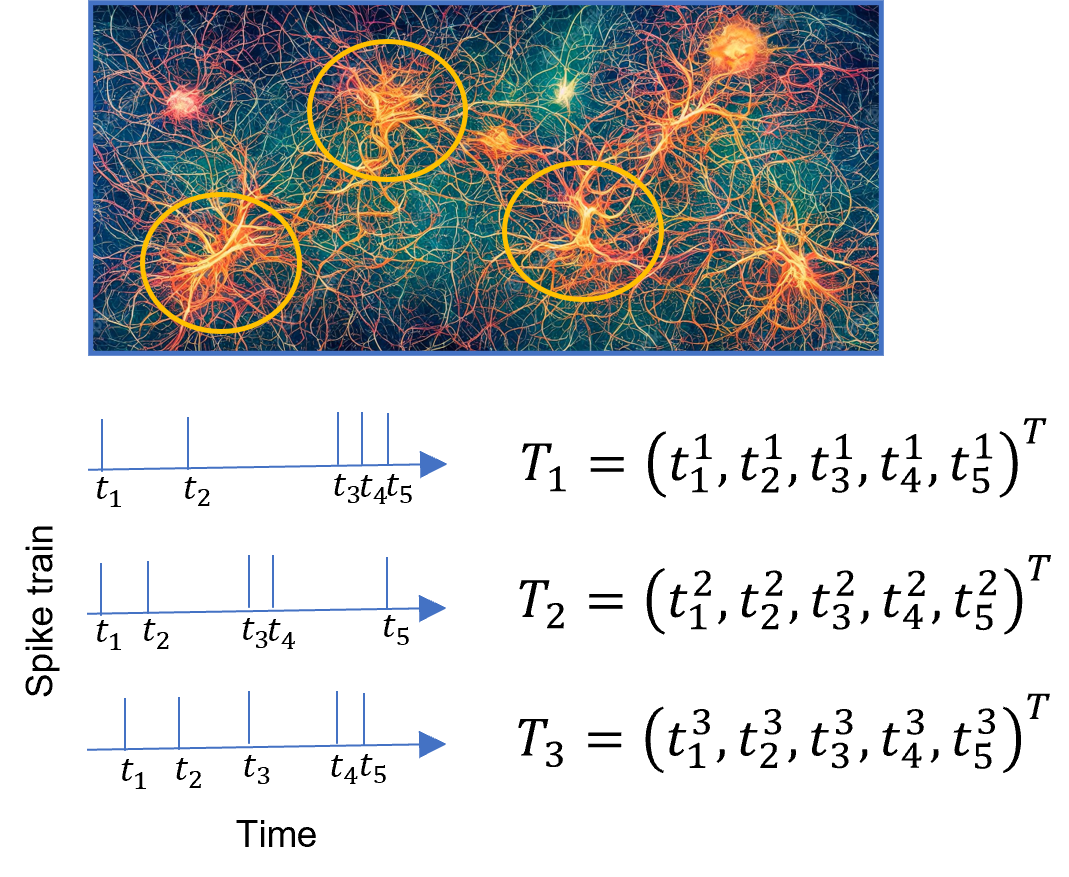
\includegraphics[height=6cm]{Random_Vector_Example.png}
\end{frame}

%2
\begin{frame}
\frametitle{Joint Distribution and Densities}
$X = (X_1, ..., X_n)^T$: A random vector\newline \\
$F_x(x)$: Probability *Distribution* Function (*PDF*)\newline\\
$f_x(x)$: Probability *Density* function (*pdf*)\newline\\
\end{frame}

%3
\begin{frame}
\frametitle{Joint Distribution and Densities}
By definition, probability distribution function (PDF) is:\newline
$F_x(x) = P[X_1 \le x_1, ..., X_n\le x_n]$\newline\\
$x = (x_1, ..., x_n)$ we get:\newline\\
$F_x(x) = P[X\le x]$\newline\\
we associate the events:\newline
${X \le \infty}$ with the certain event, $F_x(\infty) = 1$,and\newline\\
${X \le -\infty}$ with the impossible event, $F_x(-\infty) = 0.$\\
\end{frame}

%4
\begin{frame}
\frametitle{Joint Distribution and Densities}
The probability *density* function is defined as:\newline\\
$f_x(x) = \frac{\partial^n{F_x(x)}}{\partial{x_1}...\partial{x_n}}$\newline\\
Equivalently we could have defined it as:\newline\\
$f_x(x) = {\lim_{\Delta x_1 \to 0,...,\Delta x_n \to 0} \frac{P[x_1<X_1\le x_1+\Delta x_1,...,x_n<X_n\le x_1+\Delta x_n]}{\Delta x_1...\Delta x_n}}$\newline\\
Therefore, \newline\\
$f_x(x) \Delta x_1...\Delta x_n \simeq {P[x_1<X_1\le x_1+\Delta x_1,...,x_n<X_n\le x_1+\Delta x_n]}$\newline\\
\end{frame}

%7
\begin{frame}
\frametitle{Joint Distribution and Densities}
pdf is defined as:\newline\\
$f_x(x) = \frac{\partial^n{F_x(x)}}{\partial{x_1}...\partial{x_n}}$\newline\\
if we integrate the equation, we obtain:\newline\\
$F_x(x) = \int_{-\infty}^{x_1}...\int_{-\infty}^{x_n} f_x(x^{'})dx_1^{'}...dx_n^{'} = \int_{-\infty}^{x} f_x(x^{'})dx^{'}$\newline\\
more generally:\newline\\
$P [B] = \int_{x \in B} f_x(x^{'})dx^{'} $, where $B \subset R^N$
\end{frame}

%8
\begin{frame}
\frametitle{Joint Distribution and Densities}
constraint: $(P[B]\neq 0)$\newline\\
conditional *PDF*: $F_{x|B}(x|B) = P[X\le x|B] = \frac{P[X\le x,B]}{P[B]}$  \newline\\

mixture *distribution* function: $F_x(x) = \sum _{i=1}^{n} F_{x|B_i}(x|B_i)P[B_i]$ \newline\\
conditional *pdf*: $f_{x|B}(x|B)=\frac{\partial^n{F_{x|B}(x|B)}}{\partial{x_1}...\partial{x_n}}$ \newline\\
mixture *density* function:$f_x(x) =\sum _{i=1}^{n} f_{x|B_i}(x|B_i)P[B_i]$\newline\\
mixture: a linear combination of marginals
\end{frame}

%9
\begin{frame}
\frametitle{Joint Distribution and Densities}
Joint distribution of *two* random vectors:\newline\\
$X= (X_1,...,X_n).T$\newline\\
$Y = (Y_1,...,Y_M).T$\newline\\
$F_{XY}(x,y) = P[X\le x,Y\le y]$\newline\\
joint density: $f_{XY}(x,y) = \frac{\partial^{n+m}F_{XY}(x,y)}{\partial{x_1}...\partial{x_n}\partial{y_1}...\partial{y_m}}$\newline\\
marginal density: $f_x(x)=\int_{-\infty}^{\infty}...\int_{-\infty}^{\infty} f_{XY}(x,y)dy_1...dy_n $\newline\\

\end{frame}

\section {Expectation Vectors and Covariance Matrices}
\begin{frame}
\frametitle{Expectation Vectors and Covariance Matrices}
The expectation of the vector $X=(X_1,...,X_n)^T$ is a vector $\mu$ whose elements are given by\newline\\
$\mu_i = \int_{-\infty}^{\infty}...\int_{-\infty}^{\infty} x_if_x(x_1,...,x_n)dx_1...dx_n.$
\end{frame}



\section{Properties of Covariance Matrices}
\begin{frame}
\frametitle{Properties of Covariance Matrices}
This is ...
\end{frame}


\section {The Multidimensional Gaussian Law}
\begin{frame}
\frametitle{The Multidimensional Gaussian Law}
This is ...
\end{frame}


\section{Distribution of the Sample Mean}
\begin{frame}
\frametitle{Distribution of the Sample Mean}
This is ...
\end{frame}

\section{Conditional Gaussian distributions }
\begin{frame}
\frametitle{Conditional Gaussian distributions}
This is ...
\end{frame}
\section{Marginal Gaussian distributions }
\begin{frame}
\frametitle{Marginal Gaussian distributions}
This is ...
\end{frame}


\end{document}